\section{Felix Setiawan Lase (1174026)}
\subsection{Pengertian}
Pada dasarnya istilah sistem informasi geografis adalah kombinasi dari tiga elemen utama yaitu sistem, informasi, dan geografi.
Sistem adalah kumpulan benda, ide, dan hubungan mereka dalam mencapai tujuan bersama.\hfill\break
Sistem informasi adalah sistem antara manusia dan mesin yang terintegrasi untuk menyajikan informasi untuk mendukung fungsi operasi, manajemen, dan pengambilan keputusan dalam organisasi.\hfill\break
Penggunaan istilah informasi geografis menyiratkan informasi tentang tempat-tempat yang terletak di permukaan bumi. Pengetahuan tentang posisi di mana objek berada di permukaan bumi dan informasi tentang informasi dan posisi yang terkandung di permukaan bumi.
\subsection{Sejarah}
Pengenalan awal GIS tidak lepas dari kemajuan di bidang teknologi, khususnya komputer. Selama perang dunia kedua pemrosesan data mengalami kemajuan pesat terutama untuk memenuhi kebutuhan militer dalam memprediksi lintasan balistik. Pada awal 1960-an perkembangan ilmu komputer berkembang pesat dan siap digunakan untuk bidang lain di luar militer. Ahli meteorologi, geologi dan geofisika mulai menggunakan komputer dalam pembuatan peta.\hfill\break

Pada tahun 1963 di Kanada muncul CGIS (Sistem Informasi Geografis Kanada), dan kemudian menjadi GIS pertama di dunia. Dua tahun kemudian di Amerika Serikat mengoperasikan sistem serupa yang disebut MIDAS yang digunakan untuk memproses data sumber daya alam.
\subsection{Koordinat}
Koordinat adalah titik yang diperoleh dari perpotongan garis lintang (garis lintang) dengan garis bujur (garis bujur) sehingga akan menunjukkan lokasi di suatu daerah. Secara umum koordinat dibagi menjadi Koordinat Geografis dan Universal Transver Mercator (UTM)
\subsection{Data Geospasial}
\begin{enumerate}
	\item Data global positioning system (GPS). Data GPS dikumpulkan melalui sistem navigasi radio berbasis satelit dan darat. Smartphone yang mampu GPS dapat memberikan lokasi seseorang.
	\item Data penginderaan jauh. Penginderaan jauh melibatkan instrumen khusus yang menangkap data yang dapat dikonversi menjadi bentuk digital. 
\end{enumerate}\hfill\break

Foto udara dapat digunakan untuk mengenali beberapa objek di muka bumi. Dengan menganalisis bentuk, ukuran dan warna benda-benda ini, kita dapat mengamati keberadaan tanah basah atau kering, tanaman atau penyakit yang sehat, dan sawah irigasi atau tadah hujan. Tanah basah akan lebih gelap jika dibandingkan dengan tanah kering.

Data geospasial banyak berguna, baik untuk bisnis maupun untuk pemerintah.\hfill\break

Sebagai contoh, dengan data geospasial kita dapat melihat jalan mana yang padat atau bahkan padat. Dengan mengetahui situasi ini, pihak berwenang seperti polisi dapat melakukan penanganan seperti mengalihkan arus ke rute alternatif atau menerapkan jalan satu arah.

\subsection{Link}
\begin{itemize}
	\item \href{https://youtu.be/GOjKvnfiYC8}{Lihat Disini}
\end{itemize}
\subsection{Plagiarism}
\begin{figure}[H]
	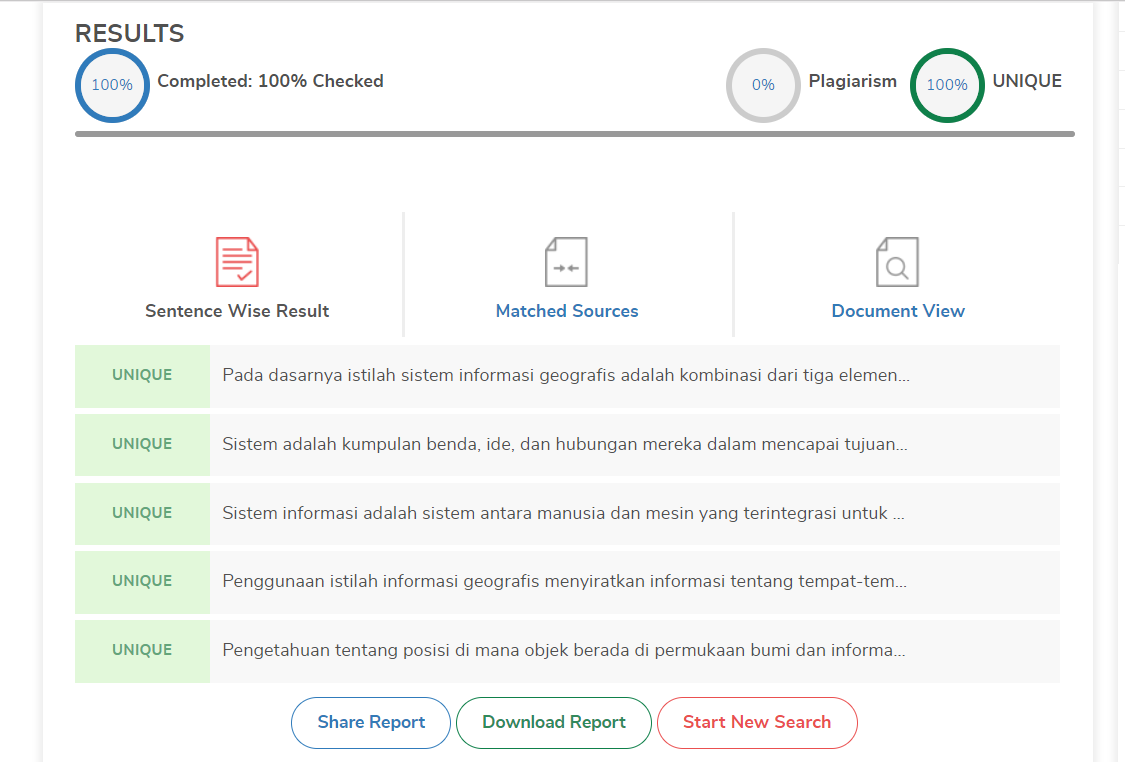
\includegraphics[width=4cm]{figures/1174026/1/1.png}
	\centering
	\caption{Bukti Tidak Melakukan Plagiat}
\end{figure}
\begin{figure}[H]
	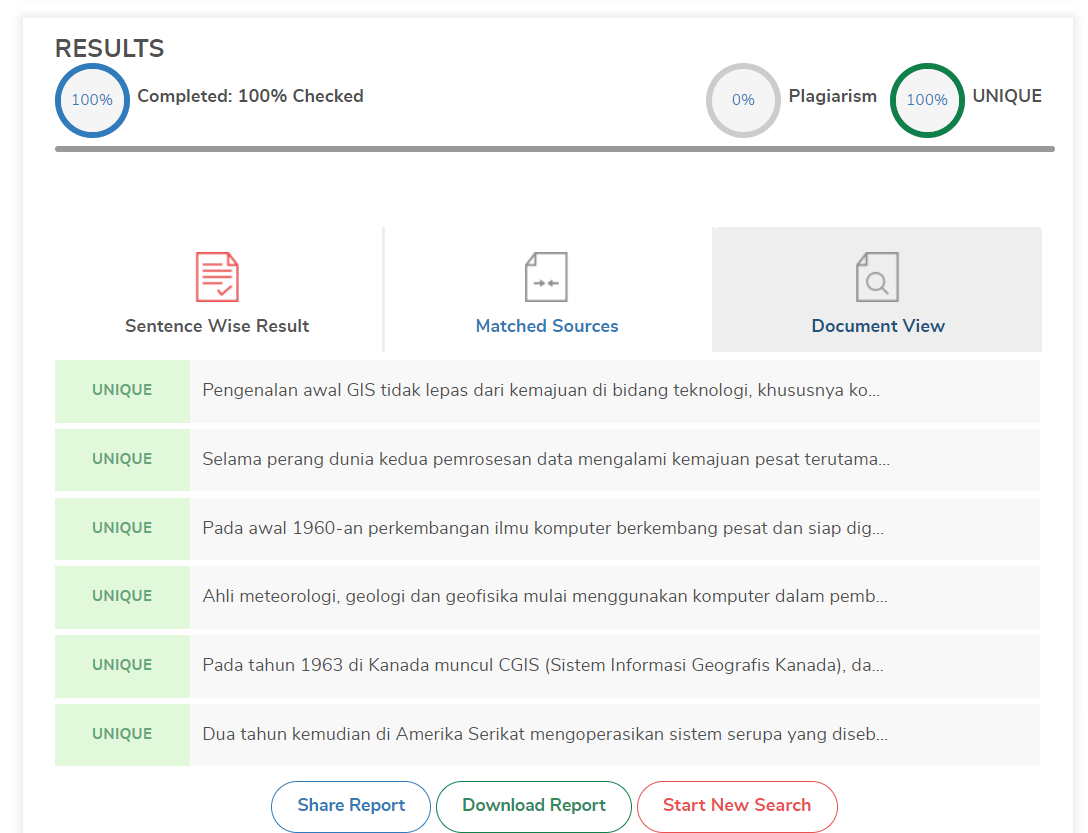
\includegraphics[width=4cm]{figures/1174026/1/2.png}
	\centering
	\caption{Bukti Tidak Melakukan Plagiat}
\end{figure}
\begin{figure}[H]
	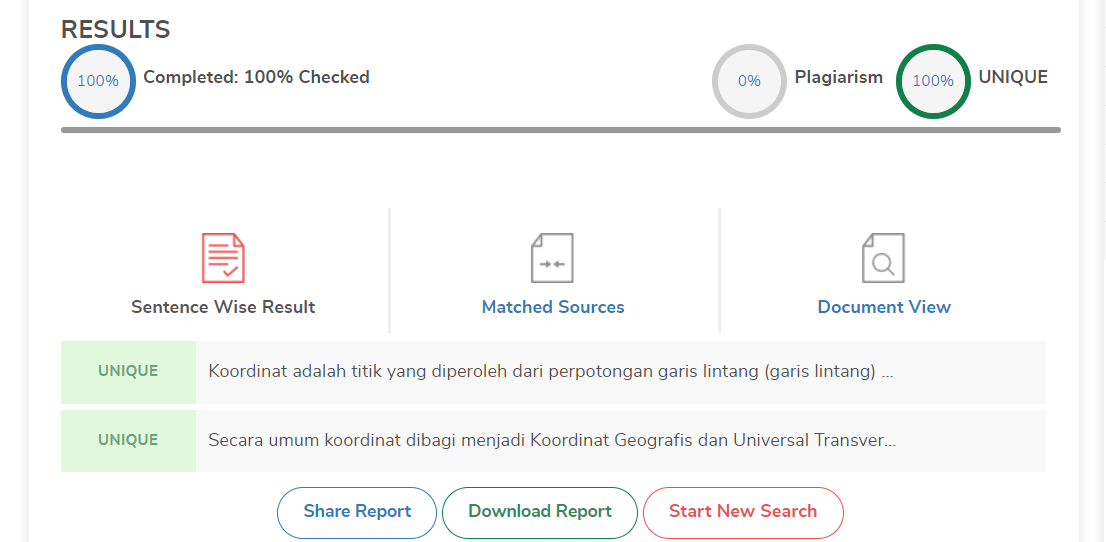
\includegraphics[width=4cm]{figures/1174026/1/3.png}
	\centering
	\caption{Bukti Tidak Melakukan Plagiat}
\end{figure}
\begin{figure}[H]
	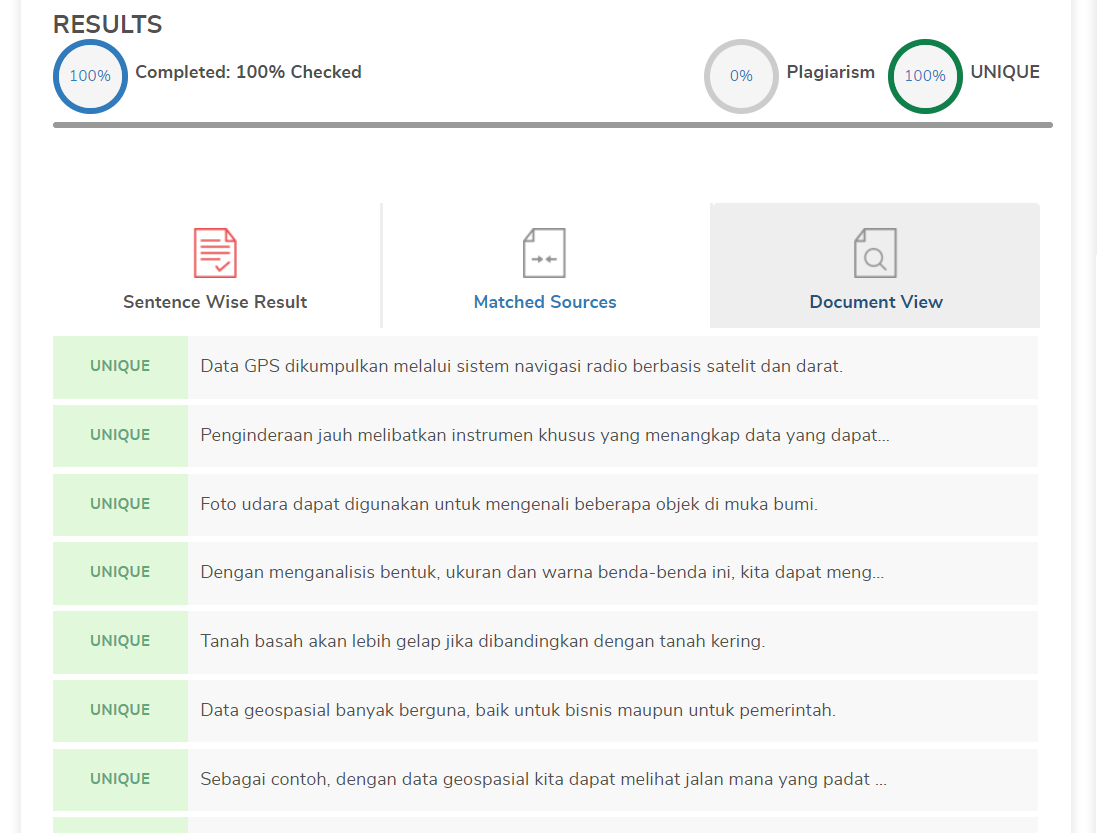
\includegraphics[width=4cm]{figures/1174026/1/4.png}
	\centering
	\caption{Bukti Tidak Melakukan Plagiat}
\end{figure}


